\section{Adminsicht}

\subsection{Installation}
Doppelt klicken.



\subsection{Start}
	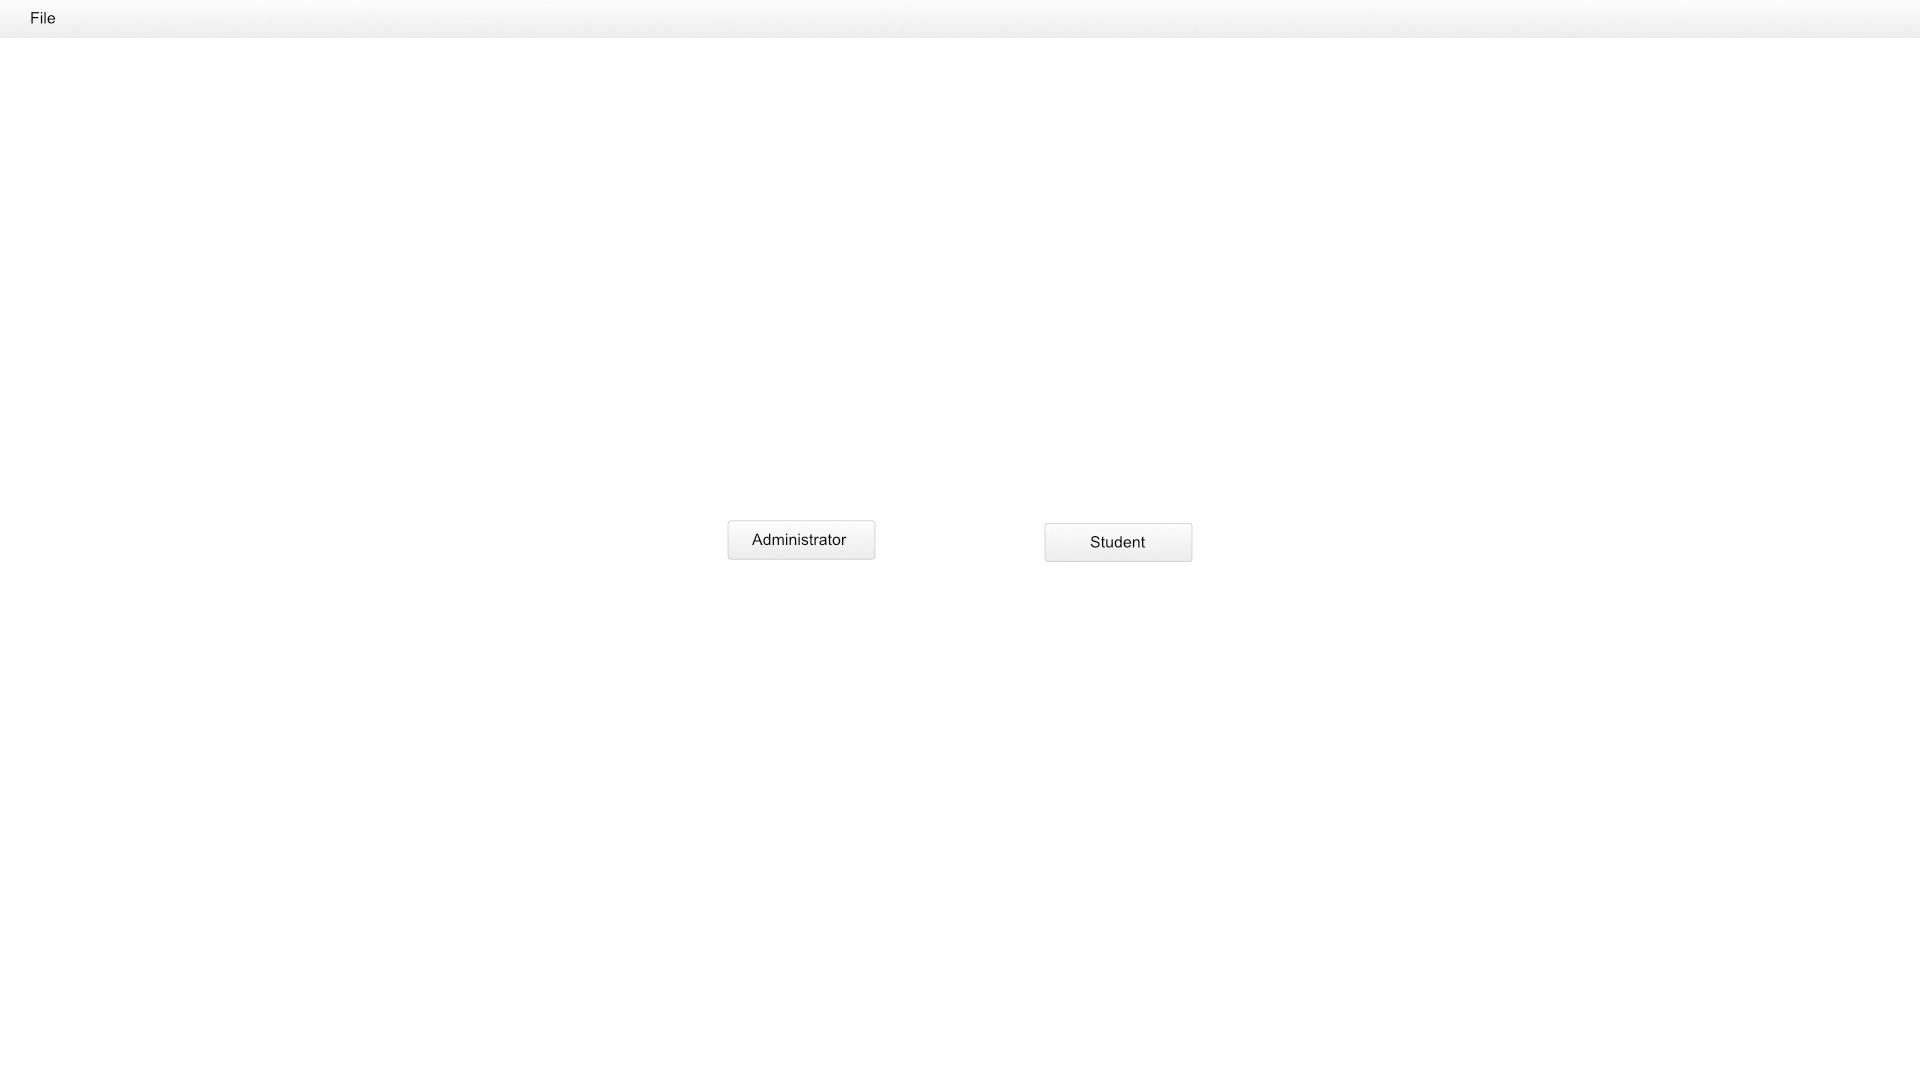
\includegraphics[width=\textwidth]{Bilder/Role-selection}
	\\
	\\
Das ist das Startfenster der Anwendung. In diesem kann der Benutzer mit einem klick auf einen der angezeigten Buttons den Zugang auswählen welchen er nutzen möchte. Für die Benutzung der Anwendung als Administrator den Button \textit{Administrator} auswählen. 



\subsubsection{Einrichten}
	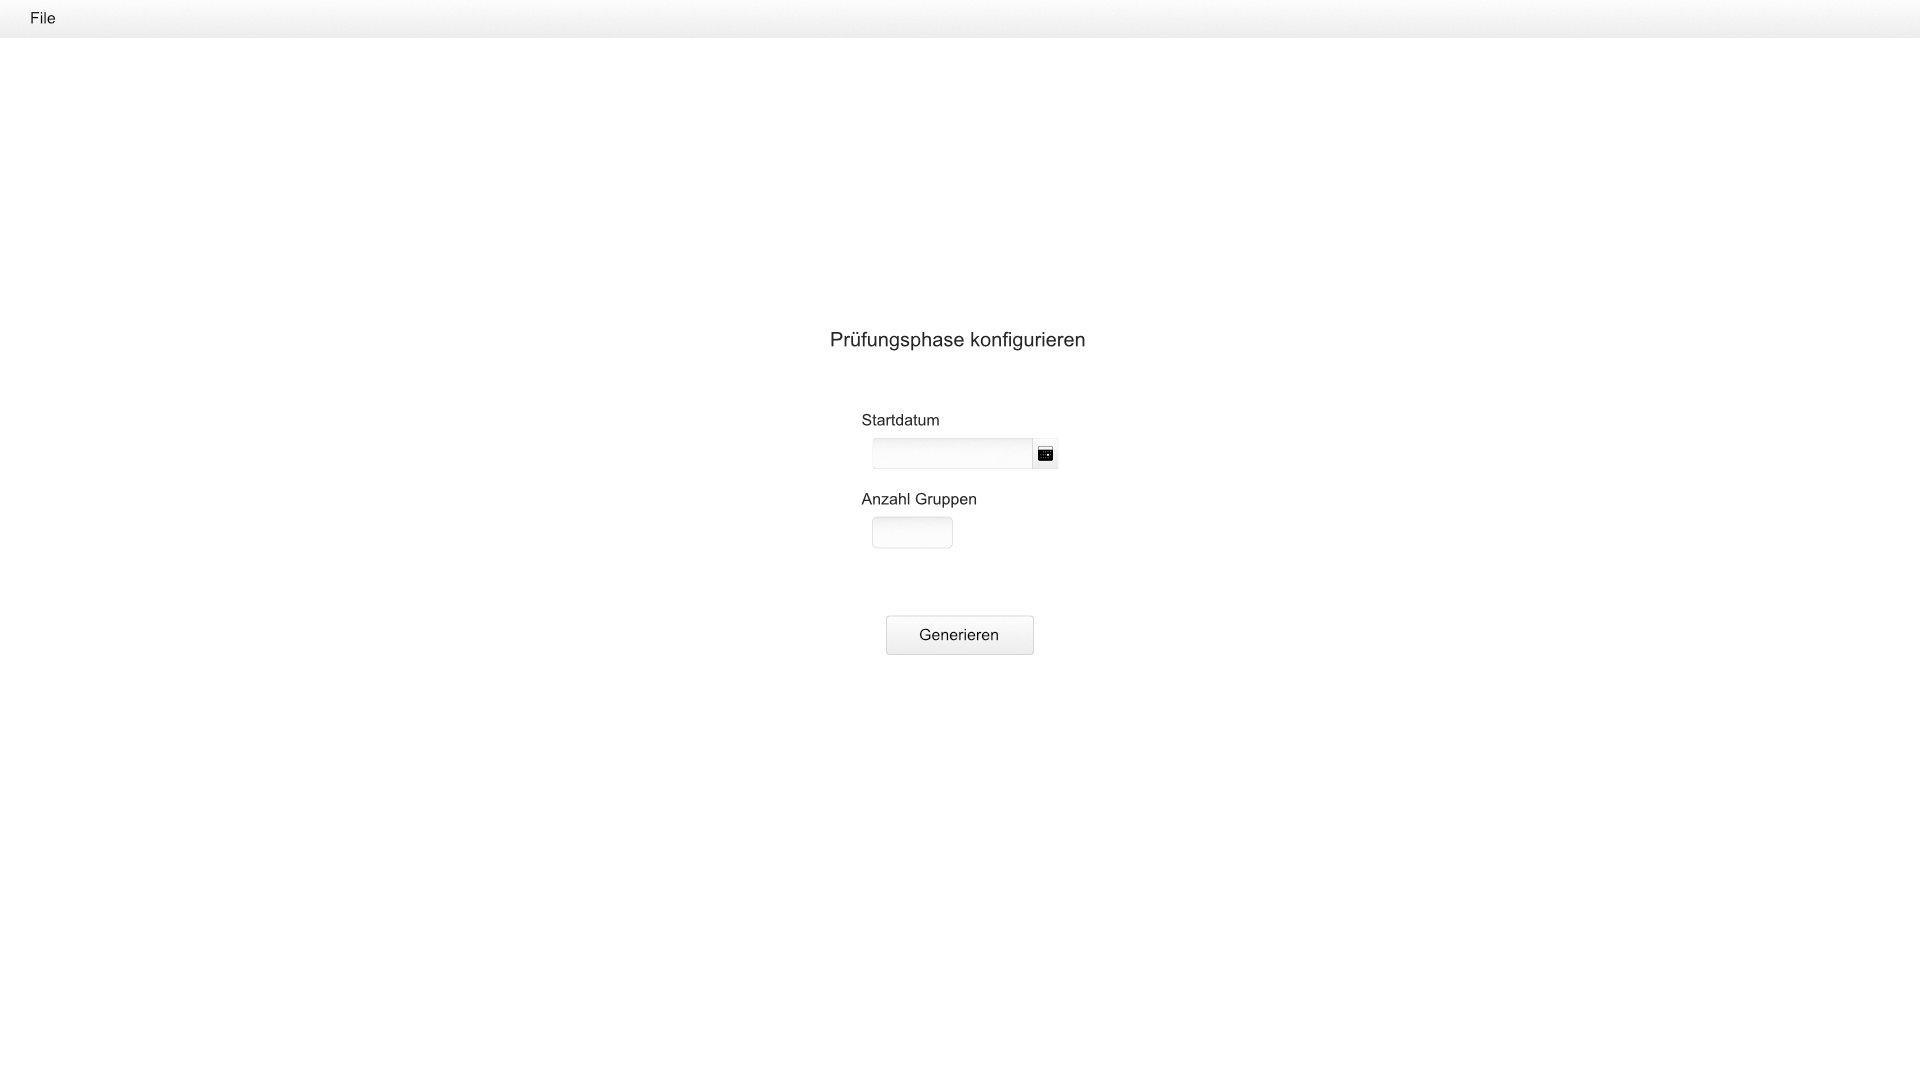
\includegraphics[width=\textwidth]{Bilder/Admin/Setup}
	\\
	\\
Die Anwendung muss von dem Administrator als ersten Schritt eingerichtet werden bevor diese von den Studenten genutzt werden kann. Dazu öffnet sich beim erstmaligen ausführen und auswählen des Button \textit{Administrator} ein Fenster. In das Textfeld \textit{Startdatum} wird der Beginn der Prüfungsphase eingetragen, wahlweise kann das Datum auch über das Kalender Icon neben dem Textfeld ausgewählt werden. In das Textfeld \textit{Anzahl der Gruppen} wird die Anzahl der Gruppen eingetragen die in der vorher festgelegten Prüfungsphase eine Präsentation halten. 
\\
\begin{wrapfigure}{R}{0.2\textwidth}
	\centering
	
\includegraphics[width=0.20\textwidth]{Bilder/Buttons/Generieren}
\end{wrapfigure}

Durch betätigen des Buttons \textit{Generieren} erstellt die Anwendung eine Listenübersicht für vier Wochen mit dem eingetragenen Datum als Startdatum.



\subsection{Tab}

\begin{wrapfigure}{R}{0.2\textwidth}
	\centering
	\includegraphics[width=0.20\textwidth]{Bilder/Admin/Group-management-btn}
\end{wrapfigure}
Es stehen zwei Tabs zur Verfügung. Diese sind oben links in der Anwendung zu finden.


\subsubsection{Gruppen}
	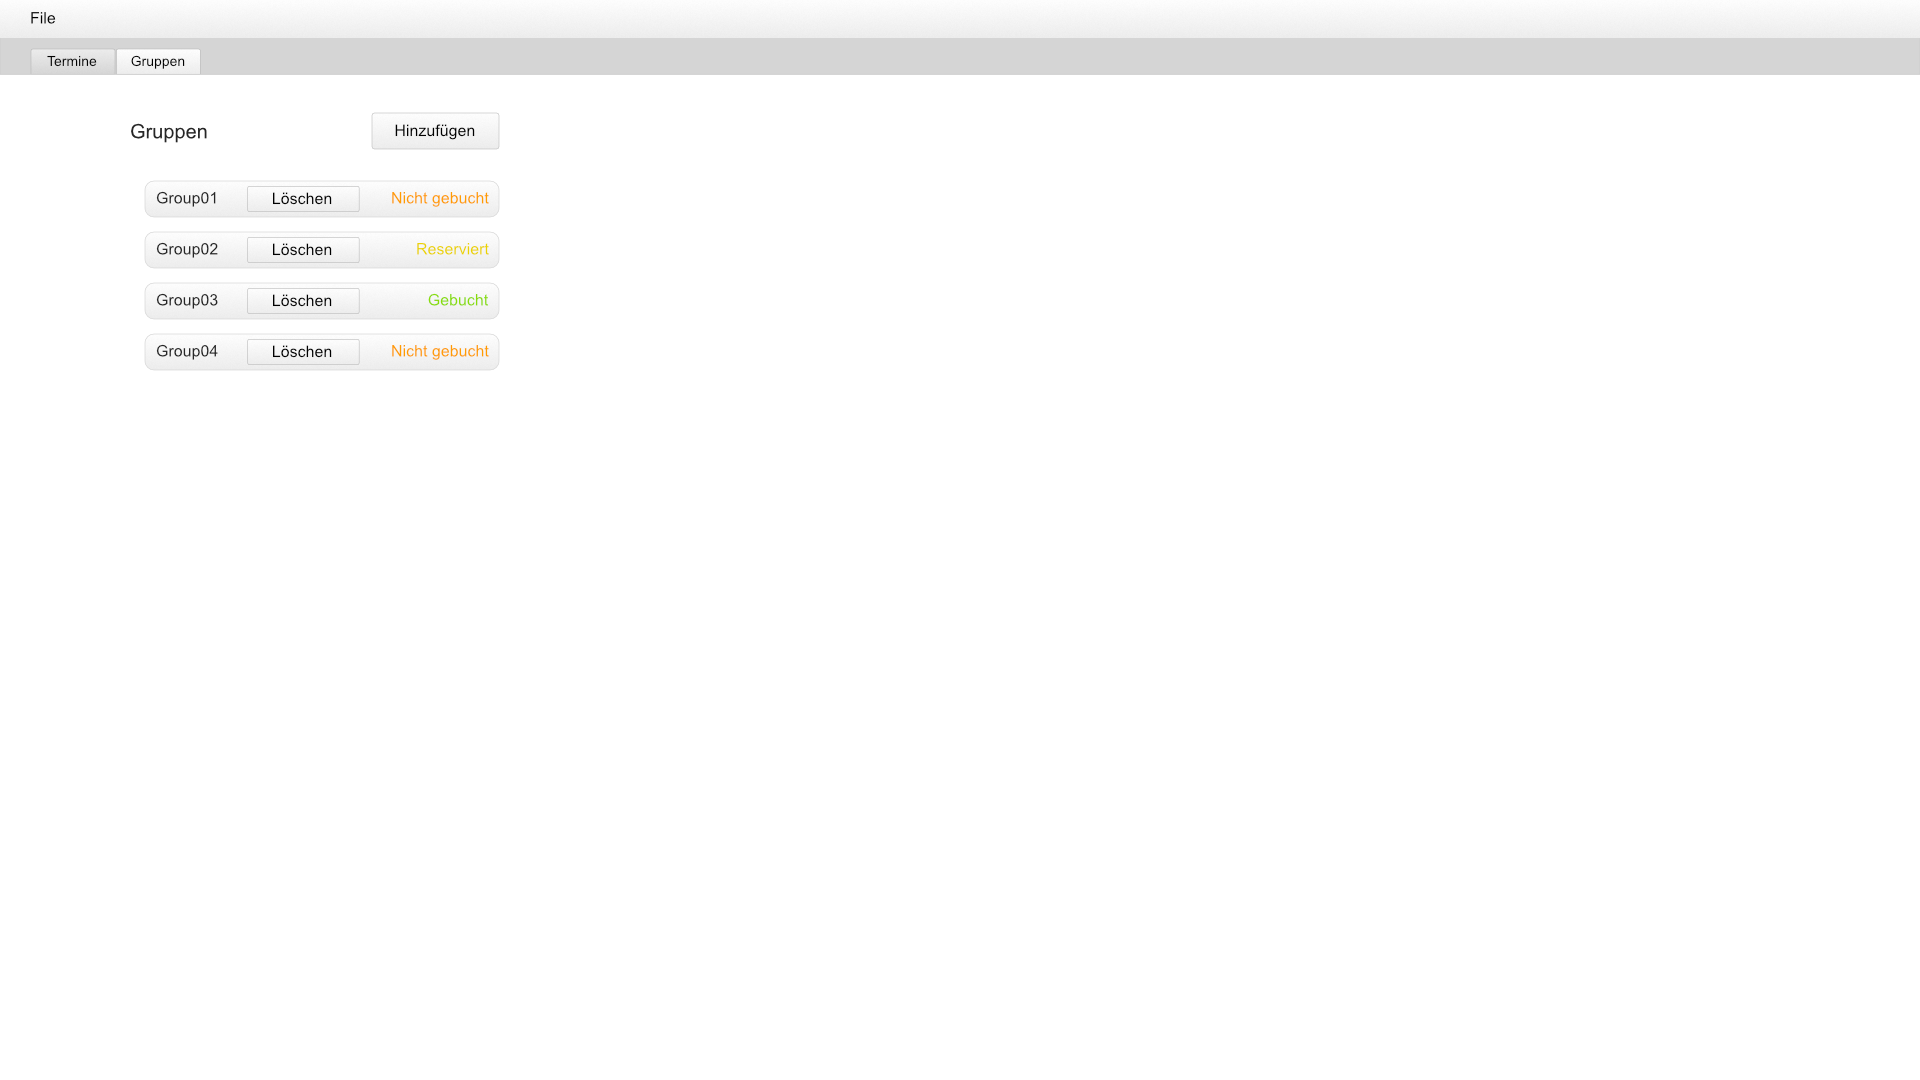
\includegraphics[width=\textwidth]{Bilder/Admin/Group-management}
	\\
	\\	
In den Tab Gruppen kann der Administrator mit dem Button \textit{Hinzufügen} eine neue Gruppe anlegen. Diese bekommt automatisch den Namen Group mit einer fortlaufenden Nummerierung.\\Mit dem Button \textit{Löschen} können bereits vorhandene Gruppen gelöscht werden auch wenn diese schon gebucht oder reserviert haben.

\subsubsection{Termine}
	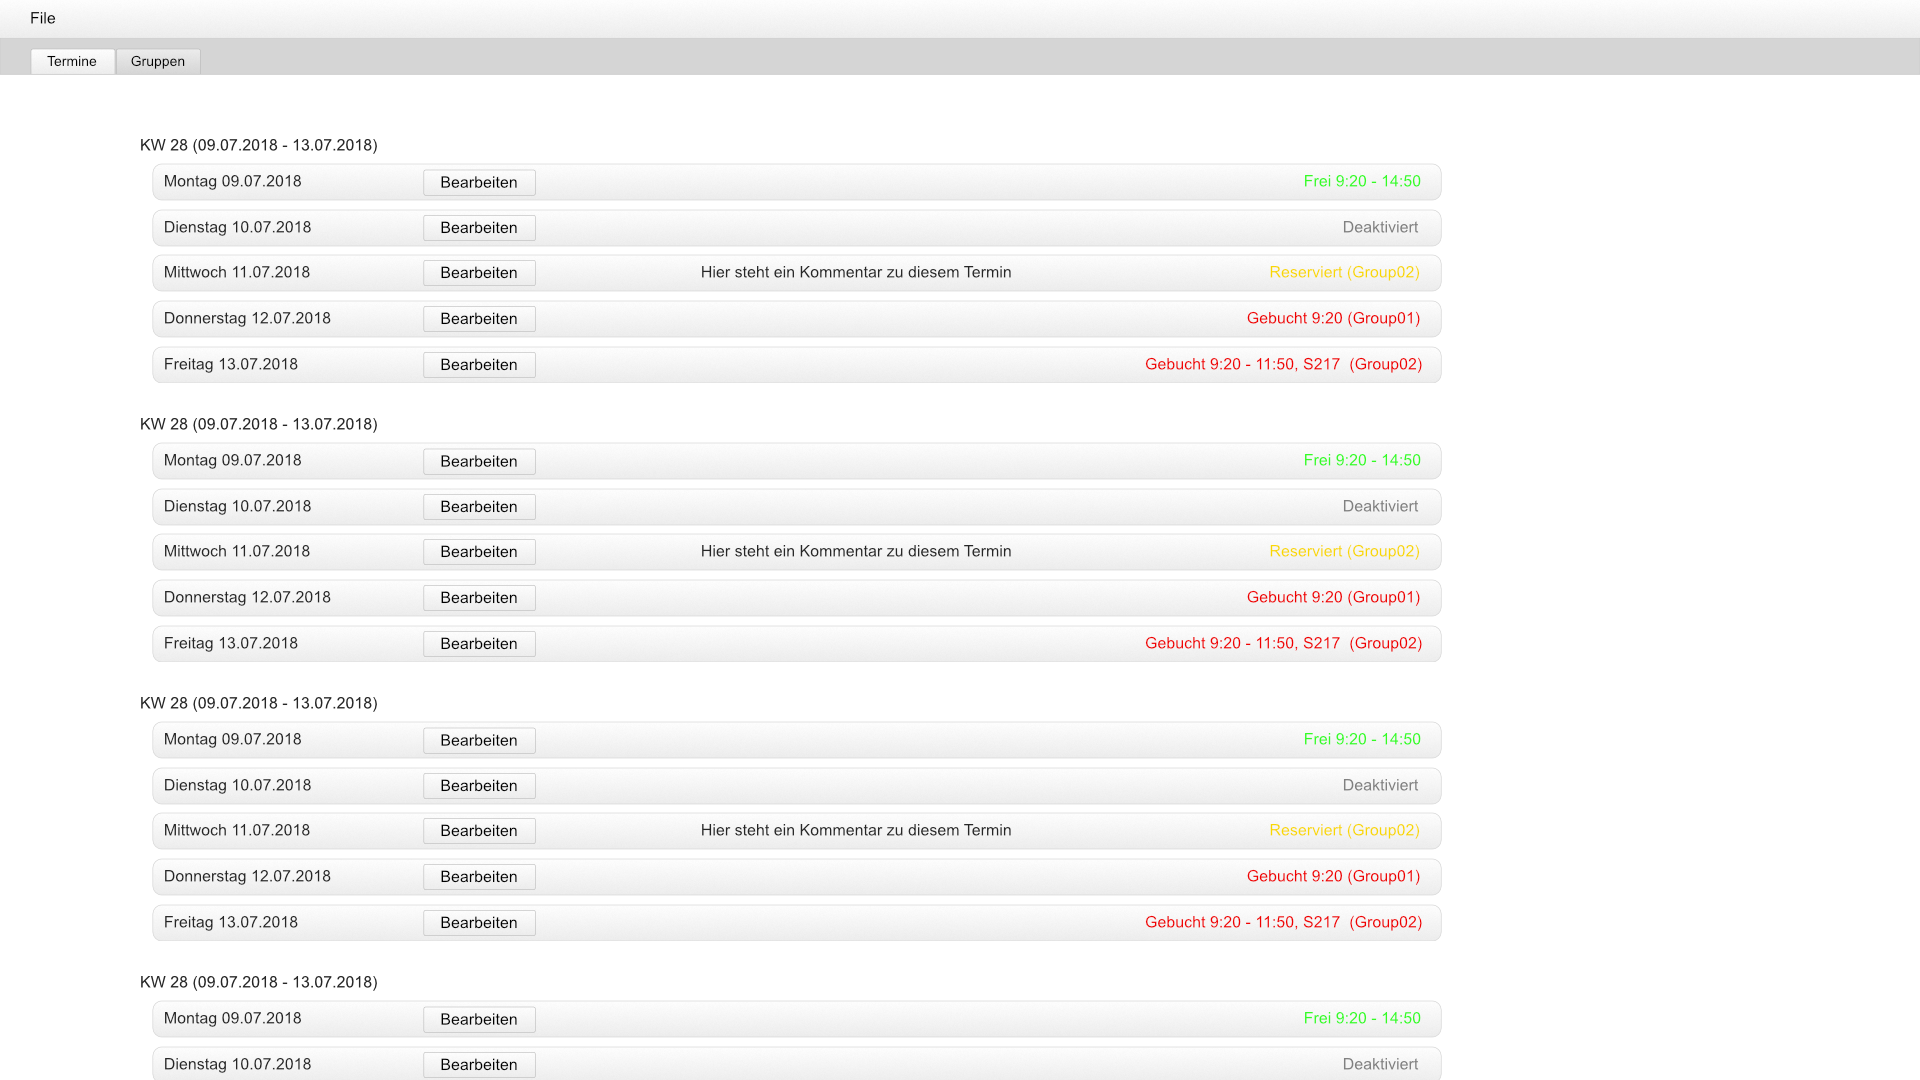
\includegraphics[width=\textwidth]{Bilder/Admin/Date-management-Admin}
	\\
	\\
In dem Tab Termine kann der Administrator die Listenübersicht der Wochen einsehen. Hier sind auch die Zustände der Tage eingetragen, sprich ob ein Tag
\begin{itemize}
	\item Aktiviert 
	\item Deaktiviert 
	\item Reserviert 
	\item Gebucht
\end{itemize}
ist.
\\ Mit dem Button \textit{Bearbeiten} können die Tage bearbeitet werden. Es öffnet sich für jeden Zustand ein entsprechendes Fenster.


\paragraph{Aktiviert}
\begin{wrapfigure}{R}{0.2\textwidth}
	\centering
	\includegraphics[width=0.4\textwidth]{Bilder/Buttons_clicked/Admin_Edit-Button-no-Booking}
\end{wrapfigure}
Ist der Tag aktiviert aber es sind keine Buchen oder Reservierungen vorhanden öffnet sich ein Fenster. In diesem kann der Administrator die Zeiträume festlegen in welchen eine möglich ist. 
\\Mit dem Button \textit{Deaktivieren} kann der Tag deaktiviert werden. Dies ist immer möglich auch wenn eine Reservierung oder eine Buchung vorhanden ist.


\paragraph{Deaktiviert}
Ist ein Tag deaktiviert kann dieser mit klicken des Buttons \textit{Bearbeiten} und daraufhin mit betätigen des Buttons \textit{Aktivieren} wieder aktiv geschaltet werden.
\\

\paragraph{Reserviert}
\begin{wrapfigure}{R}{0.2\textwidth}
	\centering
	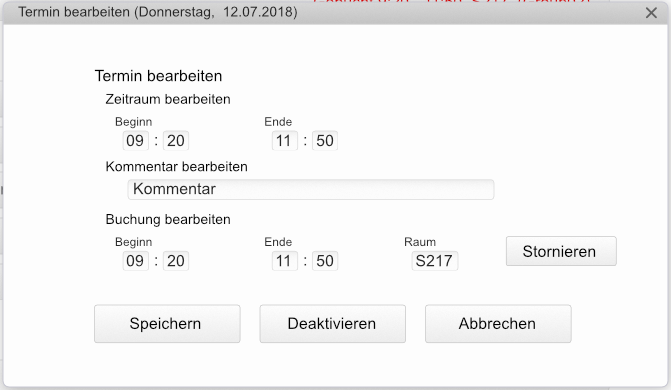
\includegraphics[width=0.4\textwidth]{Bilder/Buttons_clicked/Admin_Edit-Button-Booking}
\end{wrapfigure}
Wenn eine Reservierung vorhanden ist kann der Tag wie oben beschrieben bearbeitet werden. Zusätzlich kann der Administrator über den Button \textit{Stornieren} die Reservierung entfernen.

\paragraph{Gebucht}
Ist eine Buchung vorhanden kann diese wie oben Beschreiben storniert werden. Des Weiteren kann unter dem Abschnitt \textit{Buchung bearbeiten} eine konkrete Zeit und der Raum für die Präsentation eingetragen werden.  

\subsubsection{Speichern}
Mit klicken des Buttons \textit{Speichern} werden alle eintrage und Änderungen gespeichert und übernommen 
